\documentclass[border=4pt]{standalone}
\usepackage{amsmath,amssymb,amsfonts}
\usepackage{xcolor,colortbl,array,booktabs,multirow}
\usepackage{tikz}
\usetikzlibrary{arrows, automata, backgrounds, calendar, chains, decorations,
    matrix, mindmap, patterns, petri, positioning, shadows, shapes.geometric,
    trees, shapes, decorations.pathreplacing, calc, tikzmark, arrows.meta}
\newcommand{\st}{\text{ s.t. }}
\newcommand{\x}{\mathbf{x}}
\renewcommand{\b}{\mathbf{b}}
\newcommand{\A}{\mathbf{A}}
\newcommand{\R}{\mathbb{R}}
\newcommand{\RR}{\mathbb{R}}
\newcommand{\Z}{\mathbb{Z}}
\newcommand{\ZZ}{\mathbb{Z}}
\begin{document}
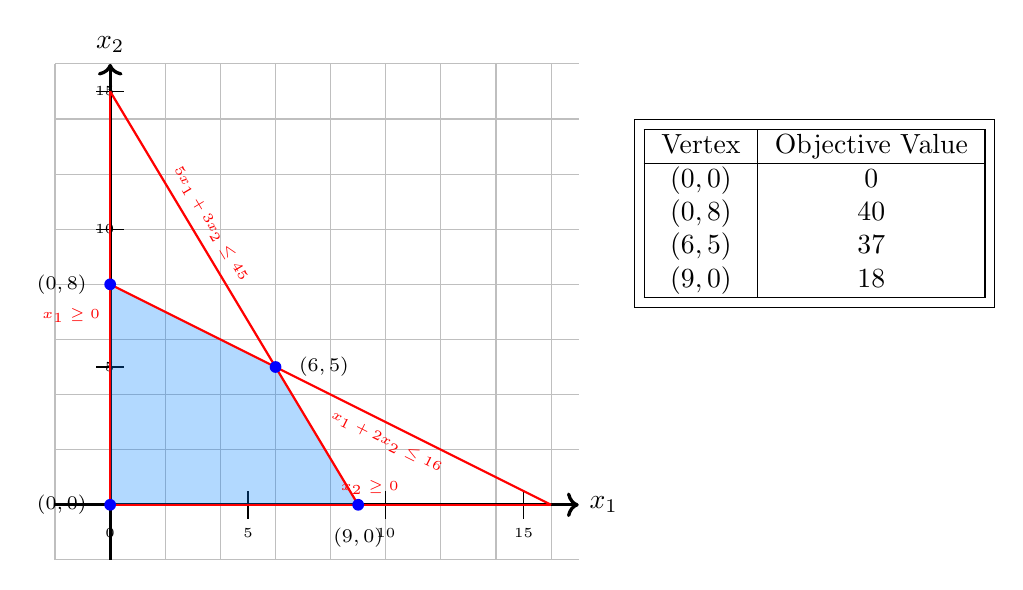
\begin{tikzpicture}[scale = 0.35]
    % Grid and axes
    \draw[gray!50, thin, step=2] (-2,-2) grid (17,16);
    \draw[very thick,->] (-2,0) -- (17,0) node[right] {$x_1$};
    \draw[very thick,->] (0,-2) -- (0,16) node[above] {$x_2$};

    % Axis labels
    \foreach \x in {0,5,10,15} \draw (\x,0.5) -- (\x,-0.5) node[below] {\tiny\x};
    \foreach \y in {0,5,10,15} \draw (-0.5,\y) -- (0.5,\y) node[left] {\tiny\y};

    % Shaded feasible region
    \fill[blue!50!cyan,opacity=0.3] (0,0) -- (0,8) -- (6,5) -- (9,0) -- cycle;

    % Constraint lines
    \draw[red,thick] (0,8) -- node[below right,sloped] {\tiny$x_1 + 2x_2 \leq 16$} (16,0);
    \draw[red,thick] (0,15) -- node[above left,sloped] {\tiny$5x_1 + 3x_2 \leq 45$} (9,0);
    \draw[red,thick] (0,0) -- node[below left] {\tiny$x_1 \geq 0$} (0,15);
    \draw[red,thick] (0,0) -- node[above right] {\tiny$x_2 \geq 0$} (16,0);

    % Vertices
    \node[blue] at (0,0) [circle,fill,inner sep=1.5pt]{};
    \node[blue] at (0,8) [circle,fill,inner sep=1.5pt]{};
    \node[blue] at (6,5) [circle,fill,inner sep=1.5pt]{};
    \node[blue] at (9,0) [circle,fill,inner sep=1.5pt]{};

    % Labels for vertices
    \node[black,anchor=east] at (-0.5,0) {\scriptsize$(0,0)$};
    \node[black,anchor=east] at (-0.5,8) {\scriptsize$(0,8)$};
    \node[black,anchor=west] at (6.5,5) {\scriptsize$(6,5)$};
    \node[black,anchor=north] at (9,-0.5) {\scriptsize$(9,0)$};
% Table within the TikZ picture
    \node[draw,fill=white,anchor=north west] at (19,14) {
        \begin{tabular}{|c|c|}
        \hline
        Vertex & Objective Value \\
        \hline
        $(0,0)$ & $0$ \\
        $(0,8)$ & $40$ \\
        $(6,5)$ & $37$ \\
        $(9,0)$ & $18$ \\
        \hline
        \end{tabular}
    };
\end{tikzpicture}
\end{document}
